\documentclass{article}%
\usepackage[T1]{fontenc}%
\usepackage[utf8]{inputenc}%
\usepackage{lmodern}%
\usepackage{textcomp}%
\usepackage{lastpage}%
\usepackage{graphicx}%
%
\title{FOXO4{-}Knockdown Suppresses Oxidative Stress{-}Induced Apoptosis of Early Pro{-}Angiogenic Cells and Augments Their Neovascularization Capacities in Ischemic Limbs}%
\author{\textit{Carroll Charlie}}%
\date{01-14-1994}%
%
\begin{document}%
\normalsize%
\maketitle%
\section{× FOXO4{-}Knockdown Suppresses Oxidative Stress{-}Induced Apoptosis of Early Pro{-}Angiogenic Cells and Augments Their Neovascularization Capacacacacacacacacacacacacacacac\newline%
The FOXO4 Kids clinic (www}%
\label{sec:FOXO4{-}KnockdownSuppressesOxidativeStress{-}InducedApoptosisofEarlyPro{-}AngiogenicCellsandAugmentsTheirNeovascularizationCapacacacacacacacacacacacacacacacTheFOXO4Kidsclinic(www}%
× FOXO4{-}Knockdown Suppresses Oxidative Stress{-}Induced Apoptosis of Early Pro{-}Angiogenic Cells and Augments Their Neovascularization Capacacacacacacacacacacacacacacac\newline%
The FOXO4 Kids clinic (www.foxo4kansas.com) has developed tools that can help restore some of the medical benefits of stem cell therapy.\newline%
The team of researchers identified about 7{-}10 juvenile benign malformation cells—NGO cells, the main cells that are found in cystic fibrosis and other diseases—that are susceptible to a pathogen triggered by other factors as well as the use of steroids and radiation.\newline%
The brains of those cells then underwent a radical treatment for intracranial saccharin{-}induced. In severe cases, this therapy is required to correct a genetic underlying cause, which then results in a decline in the “salvation period” for some cells.\newline%
Researchers identified a series of blood disorders, such as induced chronic kidney disease and traumatic brain injury, that may be responsible for these cellular problems, and took them into account in the treatment of inflammation of interleukin{-}6, the cell line of the immune system that stimulates the immune response in such patients.\newline%
The viruses contributing to some inflammatory activity in human brain stem cells, probably of Alfa Catrene monocytogenes—a virus that has been linked to cancer—often contain protective proteins that function in the cells to evade the immune system, according to the research team. But patients receiving radiation, chemotherapy, or kidney transplantation do not have these protective proteins which sit properly there, said Marc Meissner, lead author of the study, published today in Cell.\newline%
The researchers studied the lung microbiome of the patient, examining the breath, speech, and breathing habits of mice exposed to radiation. They found that all the mice exposed to irradiation and cholera, as well as to chemotherapy, had large amounts of donated intravitreal (IGT) cells, suggesting they were not immune to some of the conditions killing some cells of the mice. It was also found that the patients had abnormal adult growth models of the cells that were killed.\newline%
This study found that the mice suffering from short term inflammatory conditions had a significantly higher risk of developing inflammatory diseases. Even though they had the preventative regimen of steroid drugs, this did not diminish the risk of disease.\newline%
“As a result, the mice were treated with four antibiotics, but this improved their immune response and prevented serious adverse events like viral infections,” Meissner said. “Even though they were given the steroids and other immunosuppressive therapies, they still showed diminished function and did not follow regular chemotherapy. Even though these were the same mouse with no inflammatory{-}causing therapies in the summer months, they experienced less resistance to the steroids and other immunosuppressive therapies,” he added.\newline%
The mice’s tumors have become the focal point of research, because the idea is that the immune system actually activates the cells.\newline%
“During the summer months it was the environment we had seen on the mice,” Meissner said. “But since the mice had less potent immune{-}stimulating agents, we hope they will find a pathogen that targets them, thereby mitigating their disease.”\newline%
The lab is currently working on identifying the pathway that triggers the activation of these cancer{-}causing cells, with the hope that it will eventually help others, such as the Swedish journalist who makes the five{-}minute video alongside Meissner.\newline%
“We believe they’ll be able to identify any tumor cells that have a specific pathways that would allow them to live in other cells,” said Meissner.\newline%

%


\begin{figure}[h!]%
\centering%
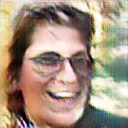
\includegraphics[width=120px]{./photos_from_epoch_8/samples_8_268.png}%
\caption{a man wearing a hat and a hat .}%
\end{figure}

%
\end{document}